\documentclass{ximera}

\begin{document}
	\author{Stitz-Zeager}
	\xmtitle{Systems of Non-Linear Equations}


\mfpicnumber{1}

\opengraphsfile{NonLinearEquations}

\setcounter{footnote}{0}

\label{NonLinearEquations}

In this section, we study systems of non-linear equations.\index{system of equations ! non-linear}   In non-linear equations, we can have variables to powers other than $1$, we can have different variables multiplied together, or variable can occur as arguments of exponential and logarithmic functions. 

Unlike the systems of linear equations for which we have developed several algorithmic solution techniques, there is no general algorithm to solve systems of non-linear equations.  Moreover, all of the usual hazards of non-linear equations like extraneous solutions and  domain restrictions are once again present.  

Along with the tried and true techniques of substitution and elimination, we shall often need equal parts tenacity and ingenuity to see a problem through to the end.  You may find it necessary to review topics throughout the text which pertain to solving equations involving the various functions we have studied thus far.  To get the section rolling we begin with a fairly routine example.

\begin{example}  \label{nonlinearex1} Solve the following systems of equations.  Verify  answers algebraically and  graphically.

\begin{multicols}{2}

\begin{enumerate}

\item  $\left\{\begin{array}{rcr}  x^2 +y^2 & = & 4 \\ 4x^2+9y^2 & = & 36 \\ \end{array} \right.$

\item  $\left\{\begin{array}{rcr}  x^2 +y^2 & = & 4 \\ 4x^2-9y^2 & = & 36 \\ \end{array} \right.$

\setcounter{HW}{\value{enumi}}
\end{enumerate}
\end{multicols}

\begin{multicols}{2}

\begin{enumerate}

\setcounter{enumi}{\value{HW}}

\item  $\left\{\begin{array}{rcr}  x^2 +y^2 & = & 4 \\ y - 2x & = & 0 \\ \end{array} \right.$

\item  $\left\{\begin{array}{rcr}  x^2 +y^2 & = & 4 \\ y  - x^2 & = & 0 \\ \end{array} \right.$

\end{enumerate}

\end{multicols}

{\sc Solution:}

\begin{enumerate}

\item  Since both equations contain $x^2$ and $y^2$ only, we can use elimination as seen in Section \ref{AppLinearSystems}:

\[ \begin{array}{ccc}

\left\{\begin{array}{lrcr} (E1) & x^2 +y^2 & = & 4 \\ (E2) & 4x^2+9y^2 & = & 36 \\ \end{array} \right.

&

\xrightarrow[\text{$-4E1 + E2$}]{\text{Replace $E2$ with}}


&

\left\{\begin{array}{lrcr} (E1) &  x^2 +y^2 & = & 4 \\ (E2) & 5y^2 & = & 20 \\ \end{array} \right.

\end{array} \]

From $5y^2 = 20$, we get $y^2 = 4$ or $y = \pm 2$.  To find the associated $x$ values, we substitute each value of $y$ into one of the equations to find the resulting value of $x$.  

Choosing $x^2 + y^2 = 4$, we find that for both $y=-2$ and $y=2$, we get $x=0$.  Our solution is thus $\{(0,2),(0,-2)\}$.  To verify these answers algebraically, we would need to show that the pair $(x,y) = (0,2)$ and $(x,y) = (0,-2)$ each satisfy \textit{both} equations.  We leave this to the reader.  

To check our answer graphically, we sketch both equations and look for their points of intersection. 

 The graph of $x^2 + y^2 = 4$ is a circle centered at $(0,0)$ with a radius of $2$.  To graph $4x^2+9y^2 = 36$, we convert to standard form  $\frac{x^2}{9} + \frac{y^2}{4} = 1$ and recognize it as an ellipse centered at $(0,0)$ with a major axis along the $x$-axis of length $6$ and a minor axis along the $y$-axis of length $4$.  
 
 We see from the graph that the two curves intersect at their $y$-intercepts only, $(0, \pm 2)$.


\item  We proceed as before to eliminate one of the variables


\[ \begin{array}{ccc}

\left\{\begin{array}{lrcr} (E1) &  x^2 +y^2 & = & 4 \\ (E2) & 4x^2-9y^2 & = & 36 \\ \end{array} \right.

&

\xrightarrow[\text{$-4E1 + E2$}]{\text{Replace $E2$ with}}


&

\left\{\begin{array}{lrcr} (E1) &  x^2 +y^2 & = & 4 \\ (E2) & -13y^2 & = & 20 \\ \end{array} \right.

\end{array} \]

Since the equation $-13y^2=20$ admits no real solution, the system is inconsistent.  To verify this graphically, we note that $x^2+y^2=4$ is the same circle as before, but when writing the second equation in standard form,  $\frac{x^2}{9} - \frac{y^2}{4} = 1$, we find a hyperbola centered at $(0,0)$ opening to the left and right with a transverse axis of length $6$ and a conjugate axis of length $4$.  

We see that the circle and the hyperbola have no points in common, hence, there are no solutions.

\[ \begin{array}{cc}

\begin{mfpic}[15]{-4}{4}{-3}{3}
\axes
\tlabel[cc](4,-0.5){\scriptsize $x$}
\tlabel[cc](0.5,3){\scriptsize $y$}
\tlabel[cc](1, 2.5){\scriptsize $(0,2)$}
\tlabel[cc](1, -2.5){\scriptsize $(0,-2)$}
\xmarks{-3,-2,-1,1,2,3}
\ymarks{-2,-1,1,2}
\tlpointsep{4pt}
\axislabels {x}{{\scriptsize $-3 \hspace{13pt}$} -3, {\scriptsize $-2 \hspace{13pt}$} -2, {\scriptsize $-1 \hspace{7pt}$} -1, {\scriptsize $1$} 1, {\scriptsize $\hspace{7pt} 2$} 2, {\scriptsize $ \hspace{9pt} 3$} 3}
\axislabels {y}{{\scriptsize $-1$} -1, {\scriptsize $1$} 1}
\penwd{1.25pt}
\point[4pt]{(0,2), (0,-2)}
\circle{(0,0),2}
\ellipse{(0,0),3,2}
\end{mfpic}

&

\hspace{1in}

\begin{mfpic}[15]{-4}{4}{-3}{3}
\axes
\tlabel[cc](4,-0.5){\scriptsize $x$}
\tlabel[cc](0.5,3){\scriptsize $y$}
\xmarks{-3,-2,-1,1,2,3}
\ymarks{-2,-1,1,2}
\tlpointsep{4pt}
\axislabels {x}{{\scriptsize $-3 \hspace{17pt}$} -3, {\scriptsize $-2 \hspace{13pt}$} -2, {\scriptsize $-1 \hspace{7pt}$} -1, {\scriptsize $1$} 1, {\scriptsize $\hspace{7pt} 2$} 2, {\scriptsize $ \hspace{9pt} 3$} 3}
\axislabels {y}{{\scriptsize $-1$} -1, {\scriptsize $1$} 1}
\penwd{1.25pt}
\circle{(0,0),2}
\arrow \reverse \arrow \parafcn{-1.15,1.15,0.1}{(3*cosh(t),2*sinh(t))}
\arrow \reverse \arrow \parafcn{-1.15,1.15,0.1}{(-3*cosh(t),2*sinh(t))}
\end{mfpic}  \\

\text{Graphs for} \quad \left\{\begin{array}{rcr}  x^2 +y^2 & = & 4 \\ 4x^2+9y^2 & = & 36 \\ \end{array} \right.

&

\hspace{.75in}

\text{Graphs for} \quad \left\{\begin{array}{rcr}  x^2 +y^2 & = & 4 \\ 4x^2-9y^2 & = & 36 \\ \end{array} \right. \\

\end{array} \]

\item  Since there are no like terms among the two equations, elimination won't work here. Instead, we proceed using substitution.

From the equation $y - 2x =0$, we get $y=2x$. Substituting this into $x^2+y^2=4$ gives $x^2+(2x)^2 = 4$.  Solving, we find  $5x^2 = 4$ or $x = \pm \frac{2 \sqrt{5}}{5}$.  

Returning to the equation we used for the substitution, $y = 2x$, we find $y = \frac{4 \sqrt{5}}{5}$ when $x = \frac{2 \sqrt{5}}{5}$, so one solution is $\left( \frac{2 \sqrt{5}}{5} , \frac{4 \sqrt{5}}{5} \right)$ and the other is   $\left( -\frac{2 \sqrt{5}}{5} , -\frac{4 \sqrt{5}}{5} \right)$.  Hence, our final answer is  $\left\{\left( \frac{2 \sqrt{5}}{5} , \frac{4 \sqrt{5}}{5} \right),  \left( -\frac{2 \sqrt{5}}{5} , -\frac{4 \sqrt{5}}{5} \right) \right\}$.  As before, we leave the algebraic check to the reader. 

The graph of  $x^2+y^2=4$ is our circle from before and the graph of $y - 2x =0$, or $y = 2x$ is a line through the origin with slope $2$.  Even though we cannot easily verify the numerical values of the points of intersection from our sketch, we can be sure there are just two solutions: one in Quadrant I and one in Quadrant III. This observation, combined with our (your) algebraic check gives us confidence our solution is correct.\footnote{Of course, we could check our answers more accurately using a graphing utility.}

\item  While it may be tempting to solve $y-x^2=0$ as $y=x^2$ and substitute, we note that this system is set up for elimination.\footnote{We encourage the reader to solve the system using substitution to see that you get the same solution.}  

\[ \begin{array}{ccc}

\left\{\begin{array}{lrcr} (E1) &  x^2 +y^2 & = & 4 \\ (E2) & y - x^2 & = & 0 \\ \end{array} \right.

&

\xrightarrow[\text{$E1 + E2$}]{\text{Replace $E2$ with}}

&

\left\{\begin{array}{lrcr} (E1) &  x^2 +y^2 & = & 4 \\ (E2) & y^2 +y  & = & 4 \\ \end{array} \right.

\end{array} \]

From $y^2 + y = 4$ we get $y^2+y-4 = 0$ which gives $y = \frac{-1 \pm \sqrt{17}}{2}$.  Due to the complicated nature of these answers, it is worth our time to make a quick sketch of both equations first to head off any extraneous solutions we may encounter.  

We see that the circle $x^2+y^2=4$ intersects the parabola $y=x^2$ exactly \textit{twice}, and both of these points have a positive $y$ value.  

Of the two solutions for $y$, only $y = \frac{-1 + \sqrt{17}}{2}$ is positive, so to get our solution, we substitute this into $y - x^2 = 0$ and solve for $x$.  We get $x = \pm \sqrt{\frac{-1 + \sqrt{17}}{2}} = \pm \frac{\sqrt{-2 + 2\sqrt{17}}}{2}$. 

Our final answer is $\left\{ \left(\frac{\sqrt{-2 + 2\sqrt{17}}}{2},\frac{-1 + \sqrt{17}}{2}\right),\left(-\frac{\sqrt{-2 + 2\sqrt{17}}}{2},\frac{-1 + \sqrt{17}}{2}\right) \right\}$.  Checking these answers algebraically amounts to a true test of anyone's algebraic mettle and as such is left to the reader.

\[ \begin{array}{cc}

\begin{mfpic}[15]{-4}{4}{-3}{3}

\axes
\tlabel[cc](4,-0.5){\scriptsize $x$}
\tlabel[cc](0.5,3){\scriptsize $y$}
\xmarks{-3,-2,-1,1,2,3}
\ymarks{-2,-1,1,2}
\tlpointsep{4pt}
\axislabels {x}{{\scriptsize $-3 \hspace{7pt}$} -3, {\scriptsize $-2 \hspace{13pt}$} -2, {\scriptsize $-1 \hspace{7pt}$} -1, {\scriptsize $1$} 1, {\scriptsize $\hspace{7pt} 2$} 2,  {\scriptsize $3$} 3}
\axislabels {y}{ {\scriptsize $1$} 1}
\penwd{1.25pt}
\point[4pt]{(0.8944, 1.7889),(-0.8944, -1.7889) }
\circle{(0,0),2}
\arrow \reverse \arrow \function{-1.5,1.5,0.1}{2*x}
\end{mfpic}

&

\hspace{1in}

\begin{mfpic}[15]{-4}{4}{-3}{3}
\axes
\tlabel[cc](4,-0.5){\scriptsize $x$}
\tlabel[cc](0.5,3){\scriptsize $y$}
\xmarks{-3,-2,-1,1,2,3}
\ymarks{-2,-1,1,2}
\tlpointsep{4pt}
\axislabels {x}{{\scriptsize $-3 \hspace{7pt}$} -3, {\scriptsize $-2 \hspace{13pt}$} -2, {\scriptsize $-1 \hspace{7pt}$} -1, {\scriptsize $1$} 1, {\scriptsize $\hspace{7pt} 2$} 2, {\scriptsize $3$} 3}
\axislabels {y}{ {\scriptsize $-1$} -1, {\scriptsize $1$} 1}
\penwd{1.25pt}
\point[4pt]{(1.2496, 1.5616),(-1.2496, 1.5616) }
\circle{(0,0),2}
\arrow \reverse \arrow \function{-1.6,1.6,0.1}{x**2}
\end{mfpic} \\

\text{Graphs for} \quad \left\{\begin{array}{rcr}  x^2 +y^2 & = & 4 \\ y-2x & = & 0 \\ \end{array} \right.

&

\hspace{1in}

\text{Graphs for} \quad \left\{\begin{array}{rcr}  x^2 +y^2 & = & 4 \\ y-x^2 & = & 36 \\ \end{array} \right. \\

\end{array} \]

\end{enumerate}

\qed

\end{example}

A couple of remarks about Example \ref{nonlinearex1} are in order.  First note that, unlike systems of linear equations, it is possible for a system of non-linear equations to have more than one solution without having infinitely many solutions.  In fact, while we characterize systems of nonlinear equations as being `consistent' or `inconsistent,' we generally don't use the labels `dependent' or `independent'.  

Secondly, as we saw with the last problem, sometimes making a quick sketch of the problem situation can save a lot of time and effort.  While in general the curves in a system of non-linear equations may not be easily visualized, it pays to take advantage when they are.  Our next example provides some considerable review of many of the topics introduced in this text.

\begin{example}  \label{nonlinearex2} Solve the following systems of equations.  Verify answers algebraically and graphically.

\begin{multicols}{3}

\begin{enumerate}

\item  $\left\{\begin{array}{rcl}  x^2 +2xy -16 & = & 0 \\ y^2 +2xy -16 & = & 0 \\ \end{array} \right.$

\item  $\left\{\begin{array}{rcl}  y+4e^{2x} & = & 1 \\y^2 + 2e^{x} & = & 1 \\ \end{array} \right.$

\item  $\left\{\begin{array}{rcl}   z(x-2) & = & x \\ yz & = & y \\ (x-2)^2+y^2 & = & 1 \end{array} \right.$


\end{enumerate}

\end{multicols}

{\bf Solution.}

\begin{enumerate}

\item  At first glance, it doesn't appear as though elimination will do us any good since it's clear that we cannot  completely eliminate one of the variables.  The alternative, however, namely solving one of the equations for one variable and substituting it into the other, is very intimidating.

Returning to elimination,  we note that it is possible to eliminate the troublesome $xy$ term, and the constant term as well. Doing so we get a more tractable relationship between $x$ and $y$:

\[ \begin{array}{ccc}

\left\{\begin{array}{lrcr} (E1) & x^2 +2xy -16 & = & 0 \\ (E2) & y^2 +2xy -16 & = & 0 \\ \end{array} \right.

&

\xrightarrow[\text{$-E1 + E2$}]{\text{Replace $E2$ with}}


&

\left\{\begin{array}{lrcr} (E1) &  x^2 +2xy -16 & = & 0 \\ (E2) & y^2 - x^2 & = & 0 \\ \end{array} \right.

\end{array} \]

We get $y^2 - x^2 = 0$ or $y = \pm x$.   Substituting $y=x$  into $E1$ we get $x^2+2x^2-16 = 0$ so that $x^2 = \frac{16}{3}$ or $x = \pm \frac{4 \sqrt{3}}{3}$.  On the other hand, when we substitute $y = -x$ into $E1$, we get $x^2 - 2x^2 - 16 = 0$ or $x^2 = -16$ which gives no real solutions.  

Substituting each of $x = \pm \frac{4 \sqrt{3}}{3}$ into $y=x$ yields the solution $\left\{\left(\frac{4 \sqrt{3}}{3},\frac{4 \sqrt{3}}{3}\right), \left(-\frac{4 \sqrt{3}}{3},-\frac{4 \sqrt{3}}{3}\right)\right\}$.  As usual, we leave it to the reader to verifying this solution algebraically.


To verify this equation graphically,  we solve $x^2 +2xy -16 = 0$ for $y$ to obtain $y = \frac{16 - x^2}{2x}$.  We produce the graph of this equation using the techniques described in  Section \ref{RationalGraphs}.  

Solving the second equation, $y^2 +2xy -16 = 0$, for $y$, however, is more complicated.  The quadratic formula  gives $y = -x \pm \sqrt{x^2+16}$ which requires Calculus or a graphing utility to graph.

As it happens, however, we don't need either because the equation $y^2+2xy-16 = 0$ can be obtained from the equation $x^2+2xy-16=0$ by interchanging `$y$' and `$x$.'  Thinking back to Section \ref{InverseFunctions}, this means we can obtain the graph of  $y^2+2xy-16 = 0$ by reflecting the graph of  $x^2+2xy-16 = 0$ across the line $y=x$.  Doing so confirms that the two graphs intersect twice: once in Quadrant I, and once in Quadrant III as required.\footnote{An amazing coincidence.  Of course, we could use a graphing utility to verify our solutions if this didn't happen to be the case.}

\begin{center}

\begin{mfpic}[15]{-5}{5}{-5}{5}
\point[2pt]{(2.3094, 2.3094),(-2.3094, -2.3094) }
\arrow \reverse \arrow \parafcn{-5,-1.5,0.1}{(t,(16-t**2)/(2*t))}
\arrow \reverse \arrow \parafcn{1.5,5,0.1}{(t,(16-t**2)/(2*t))}
\axes
\tlabel[cc](5,-0.5){\scriptsize $x$}
\tlabel[cc](0.5,5){\scriptsize $y$}
\xmarks{-4,-3,-2,-1,1,2,3,4}
\ymarks{-4,-3,-2,-1,1,2,3,4}
\tlpointsep{4pt}
\axislabels {x}{{\scriptsize $-4 \hspace{7pt}$} -4,{\scriptsize $-3 \hspace{7pt}$} -3, {\scriptsize $-2 \hspace{7pt}$} -2, {\scriptsize $-1 \hspace{7pt}$} -1, {\scriptsize $1$} 1, {\scriptsize $2$} 2, {\scriptsize $3$} 3, {\scriptsize $4$} 4}
\axislabels {y}{ {\scriptsize $-4$} -4, {\scriptsize $-3$} -3, {\scriptsize $-2$} -2, {\scriptsize $-1$} -1, {\scriptsize $1$} 1, {\scriptsize $2$} 2, {\scriptsize $3$} 3, {\scriptsize $4$} 4}
\penwd{1.5pt}
\arrow \reverse \arrow \parafcn{-5,-1.5,0.1}{((16-t**2)/(2*t),t)}
\arrow \reverse \arrow \parafcn{1.5,5,0.1}{((16-t**2)/(2*t),t)}
\end{mfpic}

The graphs of $x^2 + 2xy - 16 = 0$ and \boldmath $y^2 +2xy - 16 = 0$

\end{center}

\item  Unlike the previous problem, there seems to be no avoiding substitution and a bit of algebraic unpleasantness.  Solving $y+4e^{2x}=1$ for $y$, we get $y = 1 - 4e^{2x}$ which, when substituted into the second equation, yields $\left(1 - 4e^{2x}\right)^2 + 2e^{x} = 1$.  

After expanding and gathering like terms, we get $16e^{4x}-8e^{2x} + 2e^{x} = 0$.  Factoring gives us $2e^{x} \left(8e^{3x}-4e^{x} + 1\right) = 0$, and since $2e^{x} \neq 0$ for any real $x$, we are left with solving $8e^{3x}-4e^{x} + 1=0$.  

We have three terms, and even though this is not a `quadratic in disguise', we can benefit from the substitution $u = e^{x}$.  The equation becomes  $8u^3-4u+1=0$.  Using the techniques set forth in Section \ref{RealZeros}, we find $u = \frac{1}{2}$ is a zero and factor $8u^3-4u+1$.   We find $8u^3-4u+1=0$ is equivalent to $\left(u - \frac{1}{2}\right) \left(8u^2+4u-2\right) =0$.  So  in addition to $u = \frac{1}{2}$, we need to solve  $8u^2+4u-2=0$.

We use the quadratic formula to solve $8u^2+4u-2=0$  and find $u = \frac{-1 \pm \sqrt{5}}{4}$.  Since $u = e^{x}$, we now must solve $e^{x} = \frac{1}{2}$ and $e^{x} =  \frac{-1 \pm \sqrt{5}}{4}$.  From $e^{x} = \frac{1}{2}$, we get $x = \ln\left(\frac{1}{2}\right) = -\ln(2)$.  

As for $e^{x} =  \frac{-1 \pm \sqrt{5}}{4}$, we first note that $ \frac{-1 - \sqrt{5}}{4} < 0$, so $e^{x} =  \frac{-1 - \sqrt{5}}{4}$ has no real solutions.  We are left with $e^{x} =  \frac{-1 + \sqrt{5}}{4}$, so that $x = \ln\left(\frac{-1 + \sqrt{5}}{4}\right)$.  

We now return to $y = 1 - 4e^{2x}$ to find the accompanying $y$ values for each of our solutions for $x$:

\begin{center}
\begin{multicols}{2}

$\begin{array}{rcl}
x & = & -\ln(2):  \\
y & = & 1 - 4e^{2x}\\
  & = & 1 - 4e^{-2\ln(2)} \\
  & = & 1 - 4e^{\ln\left(\frac{1}{4}\right)} \\
  & = & 1 - 4\left(\frac{1}{4}\right) \\
  & = & 0 \\
\end{array}$



$\begin{array}{rcl}
x & =  & \ln\left(\frac{-1 + \sqrt{5}}{4}\right): \\
y & = & 1 - 4e^{2x} \\
  & = & 1 - 4e^{2\ln\left(\frac{-1 + \sqrt{5}}{4}\right)} \\
  & = & 1 - 4e^{\ln\left(\frac{-1 + \sqrt{5}}{4}\right)^2} \\
  & = & 1 - 4\left( \frac{-1 + \sqrt{5}}{4} \right)^2 \\
  & = & 1 - 4\left(\frac{3-\sqrt{5}}{8}\right) \\
  &  = & \frac{-1+\sqrt{5}}{2}\\

\end{array}$ \\


\end{multicols}

\end{center}

We get two solutions, $\left\{ (-\ln(2),0), \left(\ln\left(\frac{-1 + \sqrt{5}}{4}\right),\frac{-1+\sqrt{5}}{2}\right) \right\}$.  It is a good review of the properties of logarithms to verify both solutions algebrically, so we leave that to the reader.  

While we are able to sketch  $y = 1 - 4e^{2x}$ using the techniques in Section \ref{ExponentialFunctions},  the second equation is more difficult and  we resort to using a graphing utility.  We see the two graphs intersect at $(-0.6931,0) \approx (-\ln(2), 0)$ and $(-1.1744, 0.618) \approx  \left(\ln\left(\frac{-1 + \sqrt{5}}{4}\right),\frac{-1+\sqrt{5}}{2}\right)$.

\begin{center}

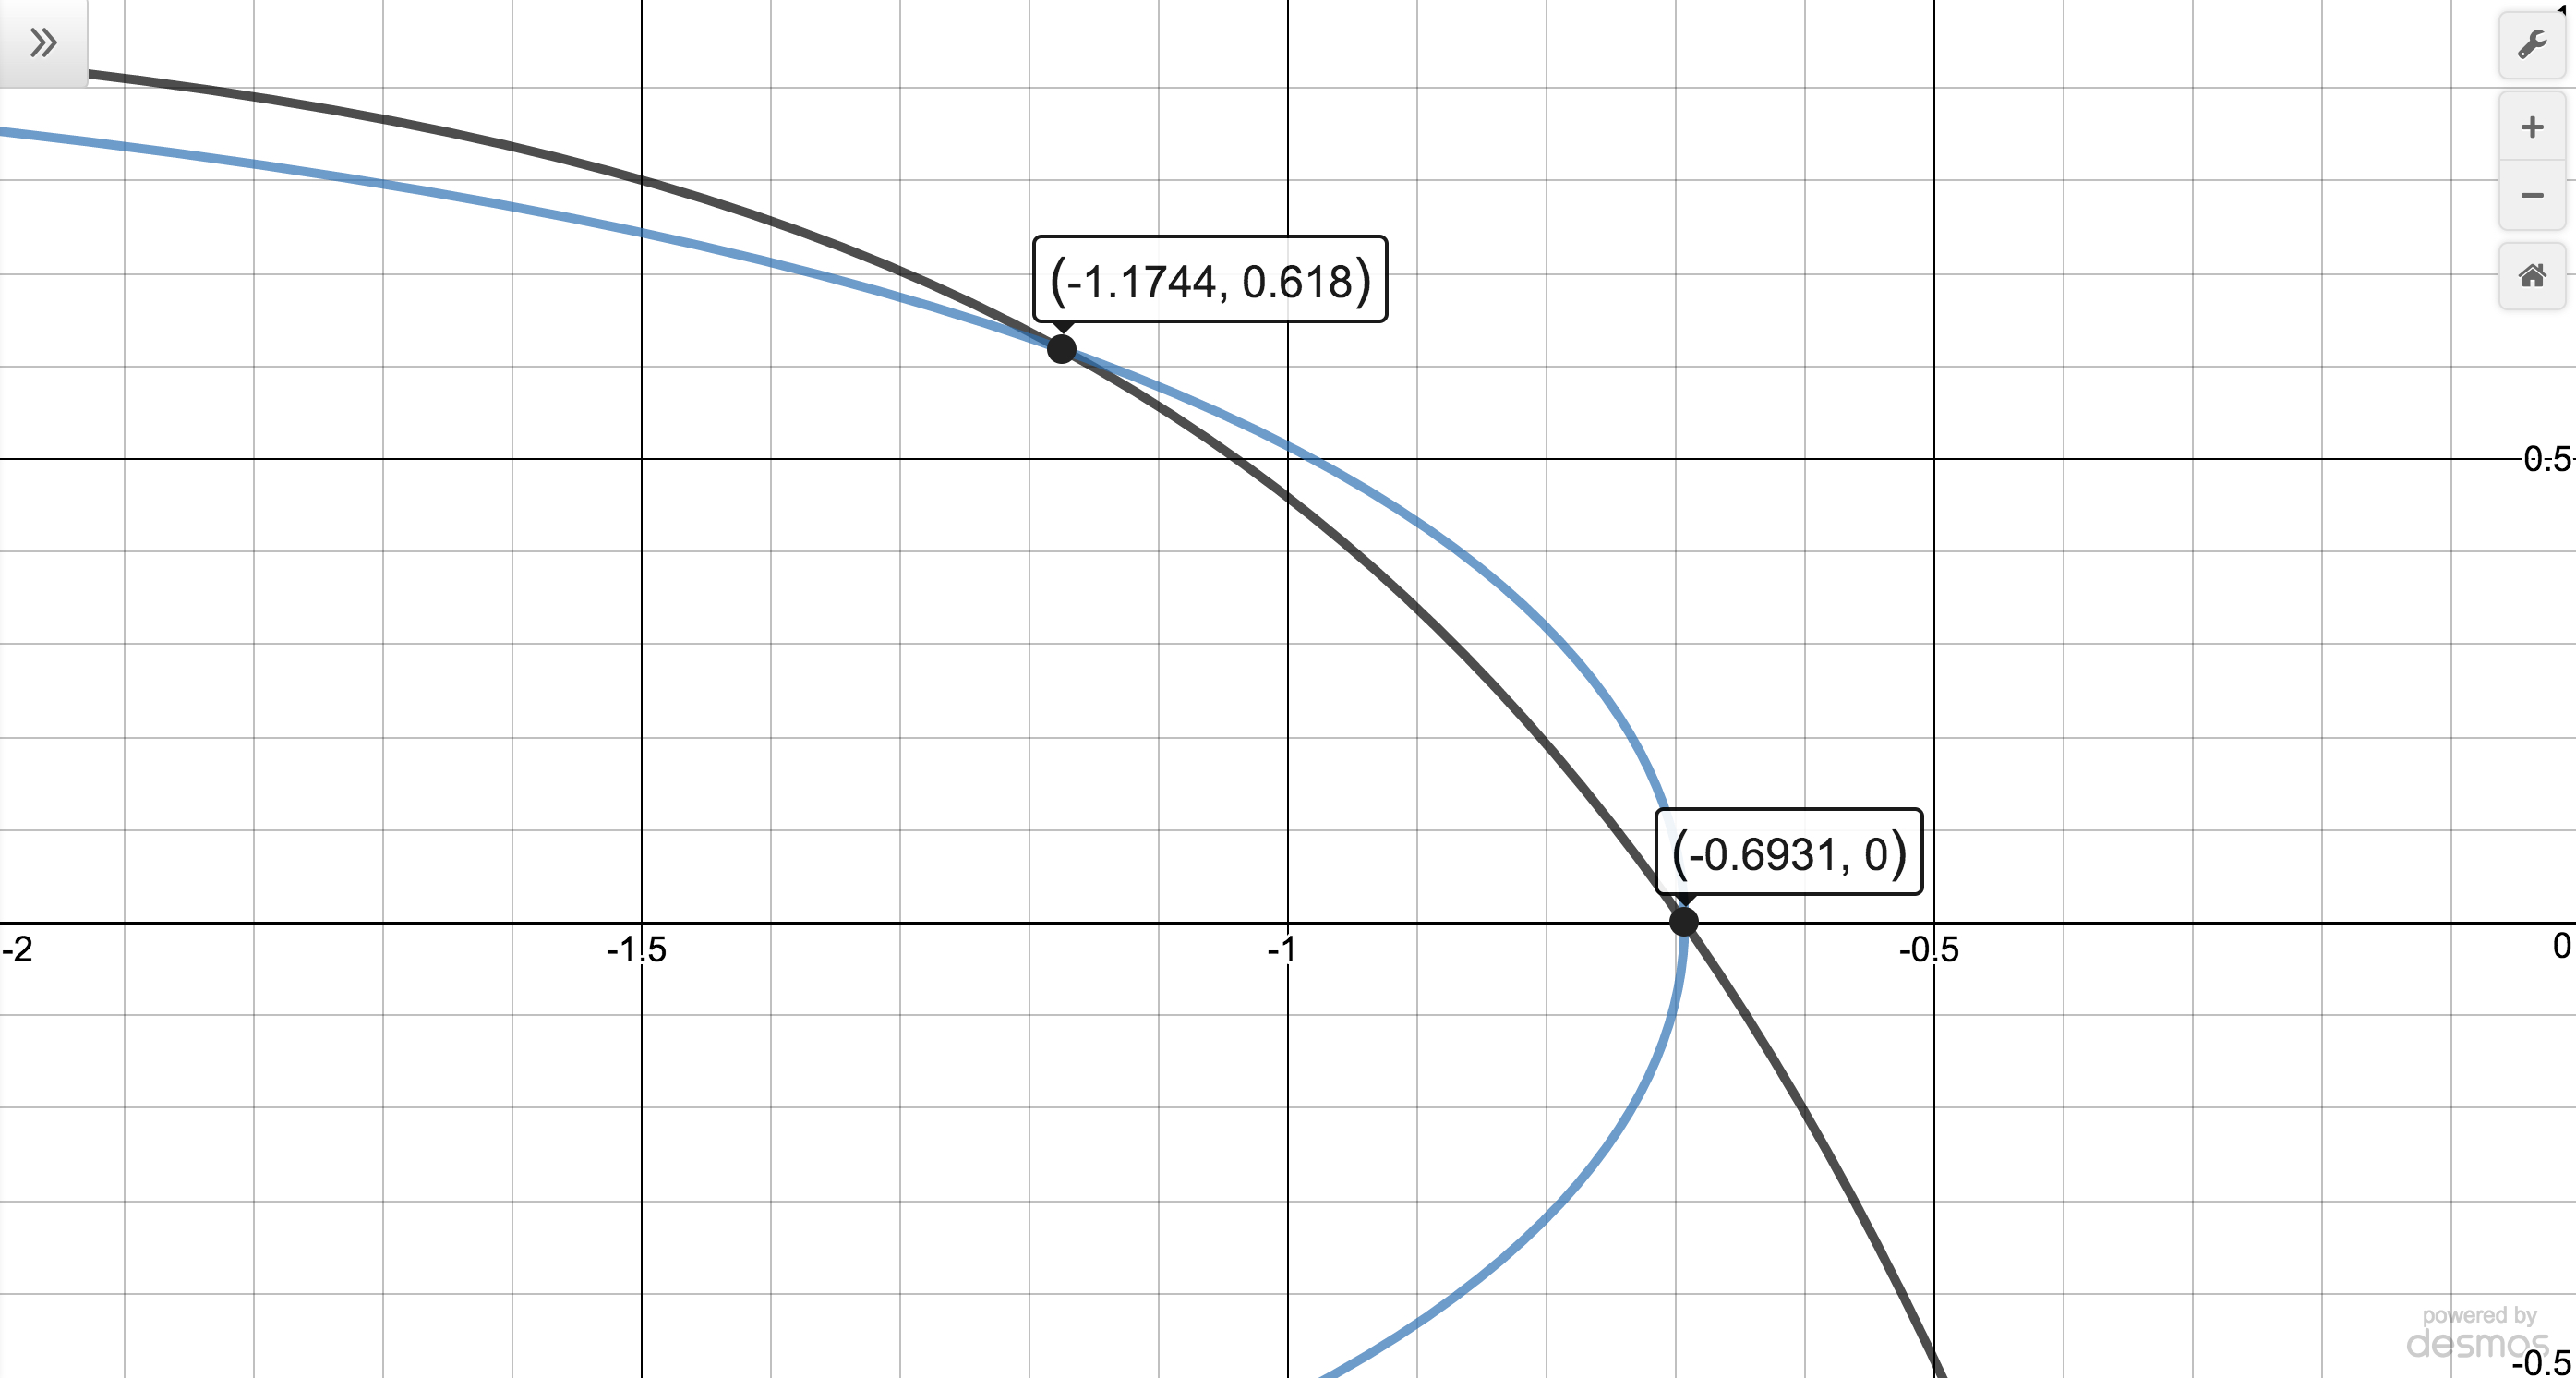
\includegraphics[width=4in]{./NonLinearEquationsGraphics/NonLinear01.jpg} 

Graphs for $\left\{\begin{array}{rcl}  y+4e^{2x} & = & 1 \\y^2 + 2e^{x} & = & 1 \\ \end{array} \right.$

\end{center}




\item  Our last system involves three variables and provides an opportunity to gain some insight on how to keep such systems organized.  Labeling the equations as before, we have

\[\left\{\begin{array}{lrcl}   E1 & z(x-2) & = & x \\ E2 & yz & = & y \\ E3 & (x-2)^2+y^2 & = & 1 \end{array} \right.\]

The easiest equation to start with appears to be $E2$.  While it may be tempting to divide both sides of $E2$ by $y$, we caution against this practice because it presupposes $y \neq 0$.  Instead, we take $E2$ and rewrite it as $yz-y = 0$ so $y(z-1) = 0$.  From this, we get two cases:  $y = 0$ or $z = 1$.

{ \sc Case 1: $y = 0$. }  Substituting $y=0$ into $E1$ and $E3$, we get 

\[\left\{\begin{array}{lrcl}   E1 & z(x-2) & = & x \\ E3 & (x-2)^2 & = & 1 \end{array} \right.\]

Solving $E3$ for $x$ gives $x = 1$ or $x=3$.  Substituting these values into $E1$ gives $z=-1$ when $x=1$ and $z = 3$ when $x=3$.  We obtain two solutions, $(1,0,-1)$ and $(3,0,3)$.

{ \sc Case 2:  $z = 1$. }  Substituting $z=1$ into $E1$ and $E3$ gives us 


\[\left\{\begin{array}{lrcl}   E1 & (1)(x-2) & = & x  \\ E3 & (x-2)^2+y^2 & = & 1 \end{array} \right.\]

Equation $E1$ gives us $x-2 = x$ or $-2 = 0$, which is a contradiction.  This means we have no solution to the system in this case, even though $E3$ is satisfied by infinitely many pairs of points $(x,y)$.  

Hence, our final answer is $\left\{ (1,0,-1), (3,0,3) \right\}$.  These points are easy enough to check algebraically in our three original equations, so that is left to the reader.  

As for verifying these solutions graphically, they require plotting surfaces in three dimensions and looking for intersection points.  While this is beyond the scope of this book, we provide a snapshot of the graphs of our three equations near one of the solution points,  $(1,0,-1)$ and $(3,0,3)$. \qed

\begin{center}

\begin{tabular}{cc}

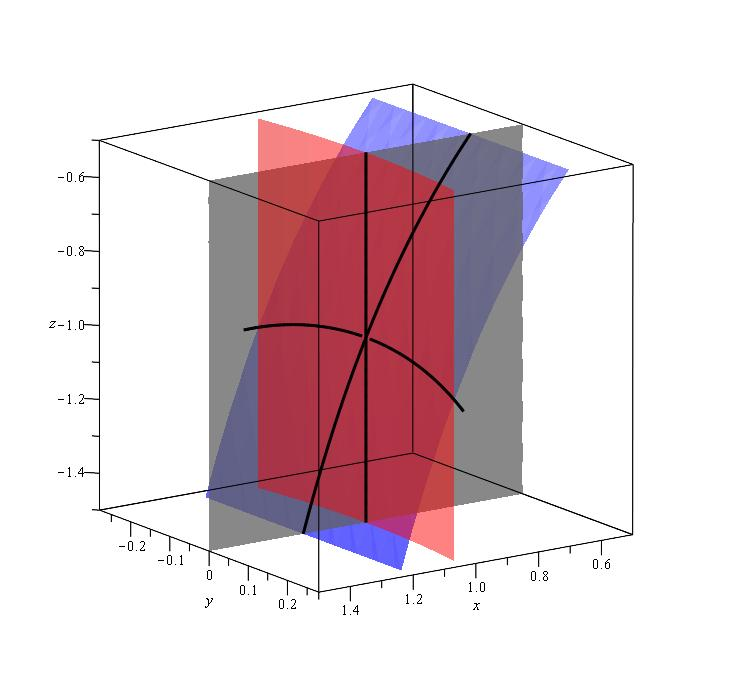
\includegraphics[height=2.25in]{./NonLinearEquationsGraphics/NonLinear03a.jpg}

&

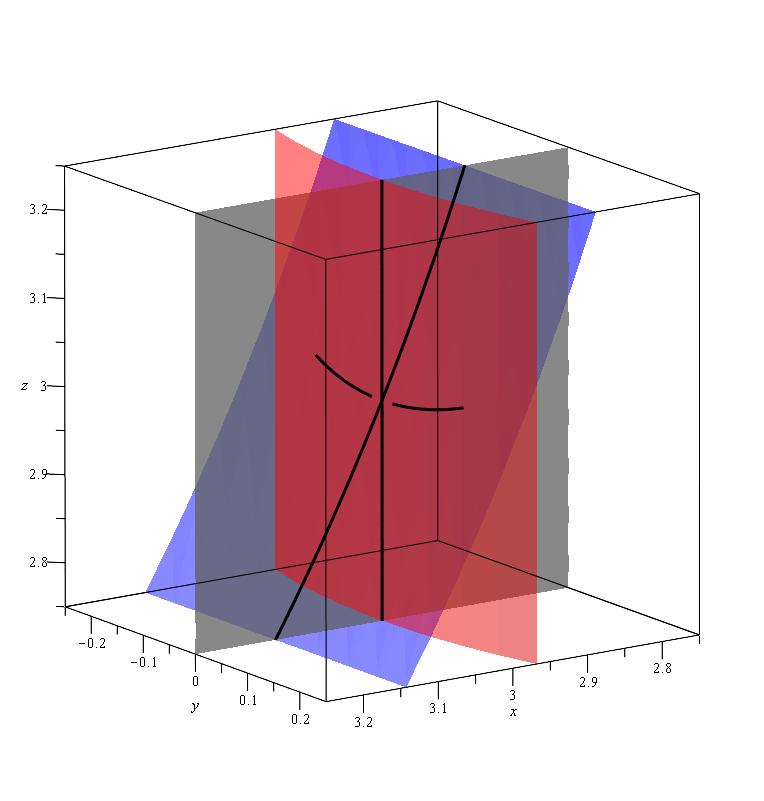
\includegraphics[height=2.25in]{./NonLinearEquationsGraphics/NonLinear03b.jpg} \\

Near $(-1,0,1)$ 

&

Near $(3,0,3)$ \\

\end{tabular}

\end{center}
\end{enumerate}


\end{example}

Example \ref{nonlinearex2} showcases some of the ingenuity and tenacity mentioned at the beginning of the section.  Sometimes you just have to look at a system the right way to find the most efficient method to solve it.  Sometimes you just have to try something.  

\smallskip

Next we explore some common application problems which give rise to systems of nonlinear equations.

\begin{example}  \label{upstreamdownstreamex}  Carl decides to explore the Meander River, the location of several recent Sasquatch sightings.  From camp, he canoes downstream five miles to check out a purported Sasquatch nest.  Finding nothing, he immediately turns around, retraces his route (this time traveling upstream), and returns to camp 3 hours after he left.  If Carl canoes at a rate  of 6 miles per hour in still water, how fast was the Meander River flowing on that day?

\smallskip

{\bf Solution.}  We are given information about distances, rates (speeds) and times.  The basic principle relating these quantities is: \[ \text{distance} = \text{rate} \cdot \text{time}\]  The first observation to make, however, is that the distance, rate and time given to us aren't `compatible':  the distance given is the distance for only \textit{part} of the trip,  the rate given is the speed Carl can canoe in still water, not in a flowing river, and  the time given is the duration of the \textit{entire} trip.  Ultimately, we are after the speed of the river, so let's call that $R$ measured in miles per hour to be consistent with the other rate given to us.  To get started, let's divide the trip into its two parts:  the initial trip downstream and the return trip upstream.  For the downstream trip, all we know is that the distance traveled is $5$ miles.

\[ \begin{array}{rcl}

\text{distance downstream} & = & \text{rate traveling downstream} \cdot \text{time traveling downstream} \\

5 \, \text{miles} & = & \text{rate traveling downstream} \cdot \text{time traveling downstream} \\ \end{array} \]

Since the return trip upstream followed the same route as the trip downstream, we know that the distance traveled upstream is also 5 miles.

\[ \begin{array}{rcl}

\text{distance upstream} & = & \text{rate traveling upstream} \cdot \text{time traveling upstream} \\

5 \, \text{miles} & = & \text{rate traveling upstream} \cdot \text{time traveling upstream} \\ \end{array} \]

We are told Carl can canoe at a  rate of $6$ miles per hour in still water.  How does this figure into the rates traveling upstream and downstream?  The speed the canoe travels in the river is a combination of the speed at which Carl can propel the canoe in still water, 6 miles per hour,  and the speed of the river, which we're calling $R$. When traveling downstream, the river is helping Carl along, so we \textit{add} these two speeds: 

\[ \begin{array}{rcl}

\text{rate traveling downstream} & = & \text{rate Carl propels the canoe} + \text{speed of the river} \\

 & = & 6 \frac{\text{miles}}{\text{hour}} + R \frac{\text{miles}}{\text{hour}} \\ \end{array} \]
 
 So our downstream speed is $(6+R) \frac{\text{miles}}{\text{hour}}$.  Substituting this into our `distance-rate-time' equation for the downstream part of the trip, we get:
 
 \[ \begin{array}{rcl}

5 \, \text{miles} & = & \text{rate traveling downstream} \cdot \text{time traveling downstream} \\ 

5 \, \text{miles} & = & (6+R) \frac{\text{miles}}{\text{hour}} \cdot \text{time traveling downstream} \\ 	\end{array} \]

 When traveling upstream, Carl works \textit{against} the current.  Since Carl must move the canoe faster than the river's speed to move upstream,  we \textit{subtract} the river's speed \textit{from} Carl's canoing speed to get:
 
 \[ \begin{array}{rcl}

\text{rate traveling upstream} & = & \text{rate Carl propels the canoe} - \text{river speed} \\

 & = & 6 \frac{\text{miles}}{\text{hour}} - R \frac{\text{miles}}{\text{hour}} \\ \end{array} \]
 
Proceeding as before, we get
 
 \[ \begin{array}{rcl}

5 \, \text{miles} & = & \text{rate traveling upstream} \cdot \text{time traveling upstream} \\ 

5 \, \text{miles} & = & (6 - R) \frac{\text{miles}}{\text{hour}} \cdot \text{time traveling upstream} \\ 	\end{array} \]
 
The last piece of information given to us is that the total trip lasted $3$ hours.  If we let $t_{\text{down}}$ denote the time of the downstream trip and $t_{\text{up}}$ the time of the upstream trip, we have:    $t_{\text{down}} + t_{\text{up}} = 3 \, \text{hours}$.  Substituting $t_{\text{down}}$ and $t_{\text{up}}$ into the `distance-rate-time' equations, we get a system of three equations in three unknowns below.  Note that since the variables in equations $E1$ and $E2$ are multiplied together, these two equations are nonlinear.

 \[\left\{\begin{array}{lrcl}   E1 & (6+R) \, t_{\text{down}} & = & 5 \\ E2 & (6-R) \, t_{\text{up}} & = & 5 \\ E3 & t_{\text{down}} + t_{\text{up}} & = & 3 \end{array} \right.\]

Since we are ultimately after $R$, we need to use these three equations to get at least one equation involving \textit{only} $R$.  We start with equation $E1$. We know that both $(6+R) \neq 0$  and  $t_{\text{down}} \neq 0$ since the product of these two quantities is $5$ and is nonzero.\footnote{This is a restatement of the Zero Product Property from Section \ref{AppRealNumberArithmetic}.}  Hence, we may solve $E1$ for $t_{\text{down}}$ by dividing both sides by the quantity $(6+R)$ to get $t_{\text{down}} = \frac{5}{6+R}$.   Similarly, we use $E2$  to get $t_{\text{up}} = \frac{5}{6-R}$. Substituting these into $E3$, we get:\footnote{The reader is encouraged to verify that the units in this equation are consistent. For starters, the units on the `3' is `hours.'} \[\dfrac{5}{6+R} + \dfrac{5}{6 - R} = 3.\] Clearing denominators, we get $5(6-R) + 5(6+R) = 3(6+R)(6-R)$ which reduces to  $R^2 = 16$.   We find $R = \pm 4$, and since $R$ represents the speed of the river, we choose $R = 4$.   On the day in question, the Meander River is flowing at a rate of $4$ miles per hour. \qed

\end{example}

One of the important lessons to learn from Example \ref{upstreamdownstreamex} is that speeds, and more generally, rates, are additive.  As we see in our next example, the concept of rate and its associated principles can be applied to a wide variety of problems - not just `distance-rate-time' scenarios.

\begin{example} \label{workex}  Working alone, Taylor can weed the garden in 4 hours.  If Carl helps, they can weed the garden in 3 hours.  How long would it take for Carl to weed the garden on his own?

\smallskip

{\bf Solution.}  The key relationship between work and time which we use in this problem is: \[\text{amount of work done} = \text{rate of work} \cdot \text{time spent working} \]

We are told that, working alone, Taylor can weed the garden in 4 hours.  In Taylor's case then: \[ \begin{array}{rcl}

\text{amount of work Taylor does} & = & \text{rate of Taylor working} \cdot \text{time Taylor spent working} \\

1 \, \text{garden} & = & (\text{rate of Taylor working}) \cdot (4 \, \text{hours}) \\ \end{array} \]

So we have that the rate Taylor works is $\frac{1 \, \text{garden}}{ 4 \, \text{hours}} = \frac{1}{4} \frac{\text{garden}}{\text{hour}}$.    We are also told that when working together, Taylor and Carl can weed the garden in just 3 hours.  We have:

\[ \begin{array}{rcl}

\text{amount of work done together} & = & \text{rate of working together} \cdot \text{time spent working together} \\

1 \, \text{garden} & = & (\text{rate of working together}) \cdot (3 \, \text{hours}) \\ \end{array} \]

From this, we find that the rate of Taylor and Carl working together is $\frac{1 \, \text{garden}}{3 \, \text{hours}} = \frac{1}{3} \frac{\text{garden}}{\text{hour}}$.   We are asked to find out how long it would take for Carl to weed the garden on his own.  Let us call this unknown $t$, measured in hours to be consistent with the other times given to us in the problem. Then:

\[ \begin{array}{rcl}

\text{amount of work Carl does} & = & \text{rate of Carl working} \cdot \text{time Carl spent working} \\

1 \, \text{garden} & = & (\text{rate of Carl working}) \cdot (t \, \text{hours}) \\ \end{array} \]

In order to find $t$, we need to find the rate of Carl working, so let's call this quantity $R$, with units $\frac{\text{garden}}{\text{hour}}$.  Using the fact that rates are additive, we have:

\[ \begin{array}{rcl}

\text{rate working together} & = & \text{rate of Taylor working} + \text{rate of Carl working} \\ [5pt]

\frac{1}{3} \frac{\text{garden}}{\text{hour}} & = & \frac{1}{4} \frac{\text{garden}}{\text{hour}} + R \frac{\text{garden}}{\text{hour}} \\ \end{array} \]

so that $R = \frac{1}{12} \frac{\text{garden}}{\text{hour}}$.  Substituting this into our `work-rate-time' equation for Carl, we get:

\[ \begin{array}{rcl}

1 \, \text{garden} & = & (\text{rate of Carl working}) \cdot (t \, \text{hours}) \\ [5pt] 

1 \, \text{garden} & = & \left(\frac{1}{12} \frac{\text{garden}}{\text{hour}} \right) \cdot (t \, \text{hours}) \\ \end{array} \]

Solving $1 = \frac{1}{12} t$, we get $t = 12$, so it takes Carl 12 hours to weed the garden on his own.\footnote{Carl would much rather spend his time writing open-source Mathematics texts than gardening anyway.} \qed

\end{example}

As is common with `word problems' like Examples \ref{upstreamdownstreamex} and \ref{workex}, there is no short-cut to the answer.  Note that in  Examples \ref{upstreamdownstreamex}, we formalized the system of non-linear equations before solving whereas in Example \ref{workex}, the system remained much in the background.  We encourage the reader to carefully think through and apply the basic principles of rate to each (potentially different!) situation.  It is time well spent.  We also encourage the tracking of units, especially in the early stages of the problem.  Not only does this promote uniformity in the units, it also serves as a quick means to check if an equation makes sense.\footnote{In other words, make sure you don't try to add apples to oranges!}

\newpage

\subsection{Exercises}
%% SKIPPED %% \documentclass{ximera}

\begin{document}
	\author{Stitz-Zeager}
	\xmtitle{TITLE}
\mfpicnumber{1} \opengraphsfile{ExercisesforNonLinearEquations} % mfpic settings added 


\label{ExercisesforNonLinearEquations}

Exercise idea:  follow up on last example and have students formalize the system there using given variables.

In Exercises \ref{solvenonlin1first} - \ref{solvenonlin1last}, solve the given system of nonlinear equations.  Sketch the graph of both equations on the same set of axes to verify the solution set. 

\begin{multicols}{3}
\begin{enumerate}

\item $\left\{\begin{array}{rcr}  x^2 - y & = & 4 \\ x^{2} + y^{2} & = & 4 \\ \end{array} \right.$ \label{solvenonlin1first}
\item $\left\{\begin{array}{rcr}  x^{2} + y^{2} & = & 4 \\ x^2 - y & = & 5 \\ \end{array} \right.$
\item $\left\{\begin{array}{rcr}  x^2+y^2 & = & 16 \\ 16x^{2} + 4y^{2} & = & 64 \\ \end{array} \right.$

\setcounter{HW}{\value{enumi}}
\end{enumerate}
\end{multicols}

\begin{multicols}{3}
\begin{enumerate}
\setcounter{enumi}{\value{HW}}

\item $\left\{\begin{array}{rcr}  x^2+y^2 & = & 16 \\ 9x^{2} - 16y^{2} & = & 144 \\ \end{array} \right.$
\item $\left\{\begin{array}{rcr}  x^2+y^2 & = & 16 \\ \frac{1}{9} y^2 - \frac{1}{16} x^2& = & 1 \\ \end{array} \right.$
\item $\left\{\begin{array}{rcr}  x^{2} + y^{2} & = & 16 \\ x-y & = & 2 \\ \end{array} \right.$ \label{solvenonlin1last}

\setcounter{HW}{\value{enumi}}
\end{enumerate}
\end{multicols}

In Exercises \ref{solvenonlin2first} - \ref{solveninlin2last}, solve the given system of nonlinear equations.  Use a graph to help you avoid any potential extraneous solutions.


\begin{multicols}{3}
\begin{enumerate}
\setcounter{enumi}{\value{HW}}


\item $\left\{\begin{array}{rcr}  x^{2} - y^{2} & = & 1 \\ x^{2} + 4y^{2} & = & 4 \\ \end{array} \right.$ \label{solvenonlin2first}
\item $\left\{\begin{array}{rcr}  \sqrt{x + 1} - y & = & 0 \\ x^{2} + 4y^{2} & = & 4 \\ \end{array} \right.$
\item $\left\{\begin{array}{rcr}  x + 2y^{2} & = & 2 \\ x^{2} + 4y^{2} & = & 4 \\ \end{array} \right.$ 

\setcounter{HW}{\value{enumi}}
\end{enumerate}
\end{multicols}

\begin{multicols}{3}
\begin{enumerate}
\setcounter{enumi}{\value{HW}}

\item $\left\{\begin{array}{rcr}  (x - 2)^{2} + y^{2} & = & 1 \\ x^{2} + 4y^{2} & = & 4 \\ \end{array} \right.$
\item $\left\{\begin{array}{rcr}  x^{2} + y^{2} & = & 25 \\ y - x & = & 1 \\ \end{array} \right.$
\item $\left\{\begin{array}{rcr}  x^{2} + y^{2} & = & 25 \\ x^{2} + (y - 3)^{2} & = & 10 \\ \end{array} \right.$

\setcounter{HW}{\value{enumi}}
\end{enumerate}
\end{multicols}

\begin{multicols}{3}
\begin{enumerate}
\setcounter{enumi}{\value{HW}}

\item $\left\{\begin{array}{rcr}  y & = & x^{3} + 8 \\ y & = & 10x - x^{2} \\ \end{array} \right. \vphantom{\left\{\begin{array}{rcr}  x^{2} + y^{2} & = & 25 \\ 4x^{2} - 9y & = & 0 \\ 3y^{2} - 16x & = & 0\end{array} \right.}$

\item $\left\{\begin{array}{rcr}  x^2 - xy & = & 8 \\  y^2 - xy & = & 8 \\ \end{array} \right. \vphantom{\left\{\begin{array}{rcr}  x^{2} + y^{2} & = & 25 \\ 4x^{2} - 9y & = & 0 \\ 3y^{2} - 16x & = & 0\end{array} \right.}$

\item $\left\{\begin{array}{rcr}  x^{2} + y^{2} & = & 25 \\ 4x^{2} - 9y & = & 0 \\ 3y^{2} - 16x & = & 0\end{array} \right.$ \label{solveninlin2last}

\setcounter{HW}{\value{enumi}}
\end{enumerate}
\end{multicols}

\begin{enumerate}
\setcounter{enumi}{\value{HW}}

\item  A certain bacteria culture follows the Law of Uninbited Growth, Equation \ref{lawofuninhibitedgrowth}.  After 10 minutes, there are 10,000 bacteria. Five minutes later, there are 14,000 bacteria.  How many bacteria were present initially?  How long before there are 50,000 bacteria?


\setcounter{HW}{\value{enumi}}
\end{enumerate}


Consider the system of nonlinear equations  below \[\left\{\begin{array}{rcr}  \dfrac{4}{x} + \dfrac{3}{y} & = & 1 \\[10pt] \dfrac{3}{x} + \dfrac{2}{y} & = & -1 \\ \end{array} \right.\]  If we let $u = \frac{1}{x}$ and $v = \frac{1}{y}$ then the system becomes \[\left\{\begin{array}{rcr}  4u + 3v & = & 1 \\ 3u + 2v & = & -1 \\ \end{array} \right.\] This associated system of linear equations can then be solved using any of the techniques presented earlier in the chapter to find that $u = -5$ and $v = 7$.  Thus $x = \frac{1}{u} = -\frac{1}{5}$ and $y = \frac{1}{v} = \frac{1}{7}$.  

\smallskip

We say that the original system is {\bf linear in form} \index{system of equations ! linear in form} because its equations are not linear but a few substitutions reveal a structure that we can treat like a system of linear equations.  Each system in Exercises \ref{linearformfirst} - \ref{linearformlast}  is linear in form.  Make the appropriate substitutions and solve for $x$ and $y$.

\begin{multicols}{3}
\begin{enumerate}
\setcounter{enumi}{\value{HW}}

\item $\left\{\begin{array}{rcr}  4x^{3} + 3\sqrt{y} & = & 1 \\ 3x^{3} + 2\sqrt{y} & = & -1  \end{array} \right.$ \label{linearformfirst}
\item $\left\{\begin{array}{rcr}  4e^{x} + 3e^{-y} & = & 1 \\ 3e^{x} + 2e^{-y} & = & -1  \end{array} \right.$
\item $\left\{\begin{array}{rcr}  4\ln(x) + 3y^{2} & = & 1 \\ 3\ln(x) + 2y^{2} & = & -1 \end{array} \right.$ \label{linearformlast}

\setcounter{HW}{\value{enumi}}
\end{enumerate}
\end{multicols}

\begin{enumerate}
\setcounter{enumi}{\value{HW}}

\item Solve the following system \[\left\{\begin{array}{rcr}  x^{2} + \sqrt{y} + \log_{2}(z) & = & 6 \\[3pt] 3x^{2} - 2\sqrt{y} + 2\log_{2}(z) & = & 5 \\[3pt] -5x^{2} + 3\sqrt{y} + 4\log_{2}(z) & = & 13 \end{array} \right.\]

\setcounter{HW}{\value{enumi}}
\end{enumerate}

\begin{enumerate}
\setcounter{enumi}{\value{HW}}


\item Systems of nonlinear equations show up in third semester Calculus in the midst of some really cool problems.  The system below came from a problem in which we were asked to find the dimensions of a rectangular box with a volume of 1000 cubic inches that has minimal surface area.  The variables $x$, $y$ and $z$ are the dimensions of the box and $\lambda$ is called a Lagrange multiplier.  With the help of your classmates, solve the system.\footnote{If using $\lambda$ bothers you, change it to $w$ when you solve the system.} \[\left\{\begin{array}{rcr}  2y + 2z & = & \lambda yz  \\ 2x + 2z & = & \lambda xz \\ 2y + 2x & = & \lambda xy \\ xyz & = & 1000 \end{array} \right.\]

\item According to Theorem \ref{realfactorization} in Section \ref{ComplexZeros}, the polynomial $p(x) = x^{4} + 4$ can be factored into the product linear and irreducible quadratic factors.  In this exercise, we present a method for obtaining that factorization.  
\label{factorpolywithnonlinear}

\begin{enumerate}

\item Show that $p$ has no real zeros.  

\item Because $p$ has no real zeros, its factorization must be of the form $(x^{2} + ax + b)(x^{2} + cx + d)$ where each factor is an irreducible quadratic.  Expand this quantity and gather like terms together.

\item Create and solve the system of nonlinear equations which results from equating the coefficients of the expansion found above with those of $x^{4} + 4$.  You should get four equations in the four unknowns $a$, $b$, $c$ and $d$.  Write $p(x)$ in factored form.

\end{enumerate}

\item Factor $q(x) = x^{4} + 6x^{2} - 5x + 6$.

\end{enumerate}

\newpage

\subsection{Answers}

\begin{multicols}{2}
\begin{enumerate}

\item $(\pm 2, 0)$, $\left(\pm \sqrt{3}, -1\right)$ \\
\begin{mfpic}[15]{-3}{3}{-5}{3}
\arrow \reverse \arrow \function{-2.5,2.5,0.1}{x**2 - 4}
\circle{(0,0),2}
\point[3pt]{(2,0), (-2,0), (1.7320,-1), (-1.7320,-1)}
\axes
\tlabel[cc](3,-0.5){\scriptsize $x$}
\tlabel[cc](0.5,3){\scriptsize $y$}
\xmarks{-2,-1,1,2}
\ymarks{-4,-3,-2,-1,1,2}
\tlpointsep{4pt}
\tiny
\axislabels {x}{{$-2 \hspace{7pt}$} -2, {$-1 \hspace{7pt}$} -1, {$1$} 1, {$2$} 2}
\axislabels {y}{{$-4$} -4,{$-3$} -3,{$-2$} -2, {$-1$} -1, {$1$} 1, {$2$} 2}
\normalsize
\end{mfpic}

\vfill

\columnbreak

\item No solution \\

\begin{mfpic}[15]{-3}{3}{-6}{3}
\arrow \reverse \arrow \function{-2.75,2.75,0.1}{x**2 - 5}
\circle{(0,0),2}
\axes
\tlabel[cc](3,-0.5){\scriptsize $x$}
\tlabel[cc](0.5,3){\scriptsize $y$}
\xmarks{-2,-1,1,2}
\ymarks{-4,-3,-2,-1,1,2}
\tlpointsep{4pt}
\tiny
\axislabels {x}{{$-2 \hspace{7pt}$} -2, {$-1 \hspace{7pt}$} -1, {$1$} 1, {$2$} 2}
\axislabels {y}{{$-4$} -4,{$-3$} -3,{$-2$} -2, {$-1$} -1, {$1$} 1, {$2$} 2}
\normalsize
\end{mfpic}

\setcounter{HW}{\value{enumi}}
\end{enumerate}
\end{multicols}

\begin{multicols}{2}
\begin{enumerate}
\setcounter{enumi}{\value{HW}}

\item  $(0, \pm 4)$ \\
\begin{mfpic}[10]{-5}{5}{-5}{5}
\ellipse{(0,0), 2, 4}
\circle{(0,0),4}
\point[3pt]{(0,4), (0,-4)}
\axes
\tlabel[cc](5,-0.5){\scriptsize $x$}
\tlabel[cc](0.5,5){\scriptsize $y$}
\xmarks{-4,-3,-2,-1,1,2,3,4}
\ymarks{-4,-3,-2,-1,1,2,3,4}
\tlpointsep{4pt}
\tiny
\axislabels {x}{{$-4 \hspace{7pt}$} -4,{$-3 \hspace{7pt}$} -3,{$-2 \hspace{7pt}$} -2, {$-1 \hspace{7pt}$} -1, {$1$} 1, {$2$} 2, {$3$} 3, {$4$} 4}
\axislabels {y}{{$-4$} -4,{$-3$} -3,{$-2$} -2, {$-1$} -1, {$1$} 1, {$2$} 2, {$3$} 3, {$4$} 4}
\normalsize
\end{mfpic}

\vfill

\columnbreak

\item  $(\pm 4,0)$ \\
\begin{mfpic}[10]{-7}{7}{-5}{5}
\arrow \reverse \arrow \parafcn{-1, 1,0.1}{(4*cosh(t), 3*sinh(t))}
\arrow \reverse \arrow \parafcn{-1, 1,0.1}{(0-4*cosh(t), 3*sinh(t))}
\circle{(0,0),4}
\point[3pt]{(4,0), (-4,0)}
\axes
\tlabel[cc](7,-0.5){\scriptsize $x$}
\tlabel[cc](0.5,5){\scriptsize $y$}
\xmarks{-6,-5,-4,-3,-2,-1,1,2,3,4,5,6}
\ymarks{-4,-3,-2,-1,1,2,3,4}
\tlpointsep{4pt}
\tiny
\axislabels {x}{{$-6 \hspace{7pt}$} -6,{$-5 \hspace{7pt}$} -5,{$-4 \hspace{7pt}$} -4,{$-3 \hspace{7pt}$} -3,{$-2 \hspace{7pt}$} -2, {$-1 \hspace{7pt}$} -1, {$1$} 1, {$2$} 2, {$3$} 3, {$4$} 4, {$5$} 5, {$6$} 6}
\axislabels {y}{{$-4$} -4,{$-3$} -3,{$-2$} -2, {$-1$} -1, {$1$} 1, {$2$} 2, {$3$} 3, {$4$} 4}
\normalsize
\end{mfpic}


\setcounter{HW}{\value{enumi}}
\end{enumerate}
\end{multicols}

\begin{multicols}{2}
\begin{enumerate}
\setcounter{enumi}{\value{HW}}

\item  $\left(\pm \frac{4 \sqrt{7}}{5}, \pm \frac{12 \sqrt{2}}{5}  \right)$ \\
\begin{mfpic}[10]{-5}{5}{-5}{5}
\arrow \reverse \arrow \parafcn{-1, 1,0.1}{(4*sinh(t), 3*cosh(t))}
\arrow \reverse \arrow \parafcn{-1, 1,0.1}{(4*sinh(t), 0-3*cosh(t))}
\circle{(0,0),4}
\point[3pt]{(2.1166,3.3941), (2.1166, -3.3941), (-2.1166,3.3941), (-2.1166,-3.3941) }
\axes
\tlabel[cc](5,-0.5){\scriptsize $x$}
\tlabel[cc](0.5,5){\scriptsize $y$}
\xmarks{-4,-3,-2,-1,1,2,3,4}
\ymarks{-4,-3,-2,-1,1,2,3,4}
\tlpointsep{4pt}
\tiny
\axislabels {x}{{$-4 \hspace{7pt}$} -4,{$-3 \hspace{7pt}$} -3,{$-2 \hspace{7pt}$} -2, {$-1 \hspace{7pt}$} -1, {$1$} 1, {$2$} 2, {$3$} 3, {$4$} 4}
\axislabels {y}{{$-4$} -4,{$-3$} -3,{$-2$} -2, {$-1$} -1, {$1$} 1, {$2$} 2, {$3$} 3, {$4$} 4}
\normalsize
\end{mfpic}

\vfill

\columnbreak

\item  $\left( 1 + \sqrt{7}, -1 + \sqrt{7}  \right)$, $\left( 1 - \sqrt{7}, -1 - \sqrt{7}  \right)$ \\
\begin{mfpic}[10]{-5}{5}{-5}{5}
\arrow \reverse \arrow \function{-3,5,0.1}{x-2}
\circle{(0,0),4}
\point[3pt]{(3.6458,1.6458), (-1.6458, -3.6458) }
\axes
\tlabel[cc](5,-0.5){\scriptsize $x$}
\tlabel[cc](0.5,5){\scriptsize $y$}
\xmarks{-4,-3,-2,-1,1,2,3,4}
\ymarks{-4,-3,-2,-1,1,2,3,4}
\tlpointsep{4pt}
\tiny
\axislabels {x}{{$-4 \hspace{7pt}$} -4,{$-3 \hspace{7pt}$} -3,{$-2 \hspace{7pt}$} -2, {$-1 \hspace{7pt}$} -1, {$1$} 1, {$2$} 2, {$3$} 3, {$4$} 4}
\axislabels {y}{{$-4$} -4,{$-3$} -3,{$-2$} -2, {$-1$} -1, {$1$} 1, {$2$} 2, {$3$} 3, {$4$} 4}
\normalsize
\end{mfpic}

\setcounter{HW}{\value{enumi}}
\end{enumerate}
\end{multicols}

\begin{multicols}{3}
\begin{enumerate}
\setcounter{enumi}{\value{HW}}

\item $\left( \pm \frac{2 \sqrt{10}}{5}, \pm \frac{\sqrt{15}}{5} \right)$
\item $(0, 1)$
\item $(0, \pm 1), \; (2, 0)$


\setcounter{HW}{\value{enumi}}
\end{enumerate}
\end{multicols}

\begin{multicols}{3}
\begin{enumerate}
\setcounter{enumi}{\value{HW}}
\item $\left( \frac{4}{3}, \pm \frac{\sqrt{5}}{3} \right)$
\item $(3, 4), \; (-4, -3)$
\item $(\pm 3, 4)$
\setcounter{HW}{\value{enumi}}
\end{enumerate}
\end{multicols}

\begin{multicols}{3}
\begin{enumerate}
\setcounter{enumi}{\value{HW}}

\item $(-4, -56), \; (1, 9), \; (2, 16)$
\item $(-2,2)$, $(2,-2)$
\item $(3, 4)$

\setcounter{HW}{\value{enumi}}
\end{enumerate}
\end{multicols}


\begin{enumerate}
\setcounter{enumi}{\value{HW}}

\item  Initially, there are $\frac{250000}{49} \approx 5102$ bacteria.  It will take $\frac{5\ln(49/5)}{\ln(7/5)} \approx 33.92$ minutes for the colony to grow to 50,000 bacteria.

\setcounter{HW}{\value{enumi}}
\end{enumerate}


\begin{multicols}{3}
\begin{enumerate}
\setcounter{enumi}{\value{HW}}

\item $\left( -\sqrt[3]{5}, 49 \right)$
\item No solution
\item $\left( e^{-5}, \pm \sqrt{7} \right)$

\setcounter{HW}{\value{enumi}}
\end{enumerate}
\end{multicols}

\begin{enumerate}
\setcounter{enumi}{\value{HW}}

\item $(1, 4, 8), \; (-1, 4, 8)$


\setcounter{HW}{\value{enumi}}
\end{enumerate}

\begin{enumerate}
\setcounter{enumi}{\value{HW}}

\item $x = 10, \; y = 10, \; z = 10, \lambda = \frac{2}{5}$

\setcounter{HW}{\value{enumi}}
\end{enumerate}

\begin{enumerate}
\setcounter{enumi}{\value{HW}}

\item \begin{enumerate} 

\addtocounter{enumii}{2}

\item $x^{4} + 4 = (x^{2} - 2x + 2)(x^{2} + 2x + 2)$

\end{enumerate}

\item $x^{4} + 6x^{2} - 5x + 6 = (x^{2} - x + 1)(x^{2} + x + 6)$

\end{enumerate}


\end{document}


\closegraphsfile

\end{document}
